\begin{figure}
  \centering
  \begin{subfigure}[b]{0.5\textwidth}
    \centering
    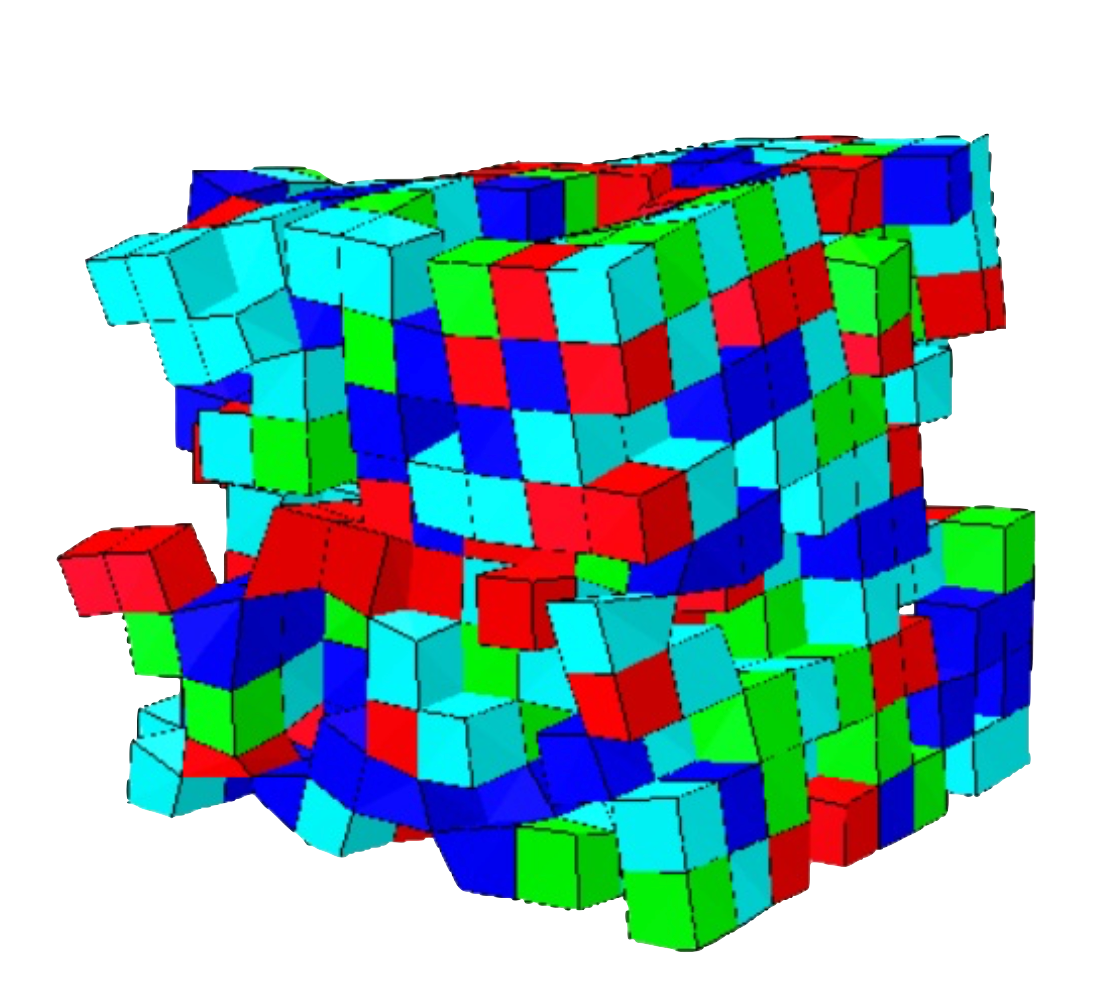
\includegraphics[width=\textwidth]{img/direct_encoding.png}
    \caption{direct encoding (low regularity)}
  \end{subfigure}%
  \hfill
  \begin{subfigure}[b]{0.5\textwidth}
    \centering
    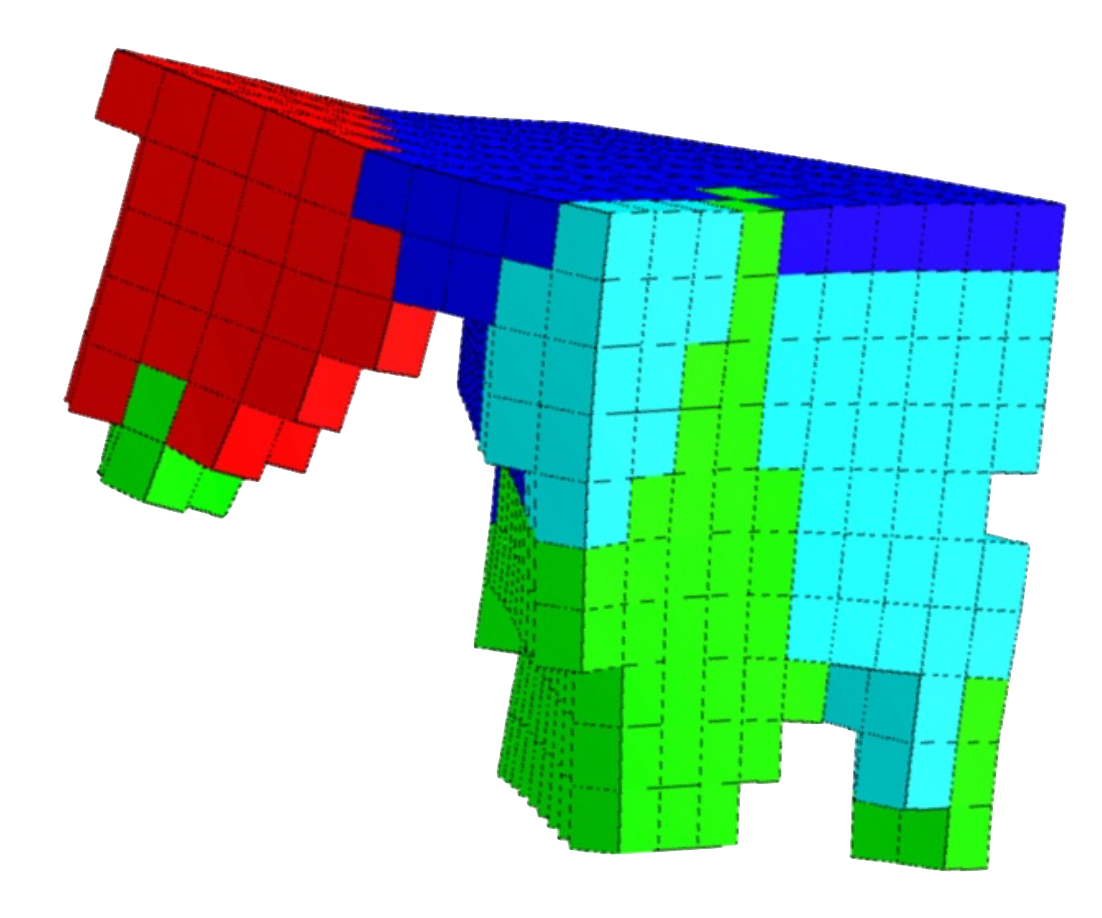
\includegraphics[width=\textwidth]{img/cppn-neat_encoded.png}
    \caption{indirect encoding (high regularity)}
  \end{subfigure}
  \captionsetup{singlelinecheck=off,justification=raggedright}
  \caption[]{Representative examples of soft robots evolved with direct and indirect representations \cite[Figures 6, 7]{Cheney2013UnshacklingEncoding}}
  \label{fig:direct_irregular_vs_indirect_regular}
\end{figure}